\section{The Nuclear Fuel Cycle}
\label{sec:nfc}

The \gls{nfc} comprizes a series of industrial processes that produce and consume nuclear fuel. Commonly, these processes are grouped into two categories (the front-end and back-end). In the \gls{usa}, we keep each of these facilities separate in the front-end of the fuel cycle in a "collect and wait" pathway \cite{cycle_risks}. In lieu of a long or interim solution for the \gls{uf}, the back end of the \gls{nfc} is collocated with the reactors that burn the fuel (with the minor exception of the consolidated storage facility in Morris Illinois). For this work, we will restrict our discussion of the fuel cycle to fuel alone, although some work has been done to consider byproducts and non-fuel wastes into related work in this field.


% differences between an open and closed fuel cycle
Nuclear fuel has the capacity to be reprocessed and recycled into a different fuel type that can produce usable power for several cycles, called a "closed" fuel cycle. As we have outlined in Figure \ref{fig:once-through}, the "open" fuel cycle is a one-time use of fuel that is then stored in a repository. The closed fuel cycle is a more sustainable option, as it reduces the amount of waste that must be stored in a repository. However, the closed fuel cycle is more expensive and has proliferation risks associated with the reprocessing of the fuel. The open fuel cycle is less expensive and has fewer proliferation risks, but it produces more waste that must be stored in a repository. The choice between an open and closed fuel cycle is a policy decision that must be made by the country that is using the fuel.


% What are the main stages of the nuclear fuel cycle?



% What processes are involved in the front-end and back-end of the nuclear fuel cycle?


% What technologies are used in uranium mining, milling, conversion, and enrichment?



\begin{figure}[h]
   \centering
   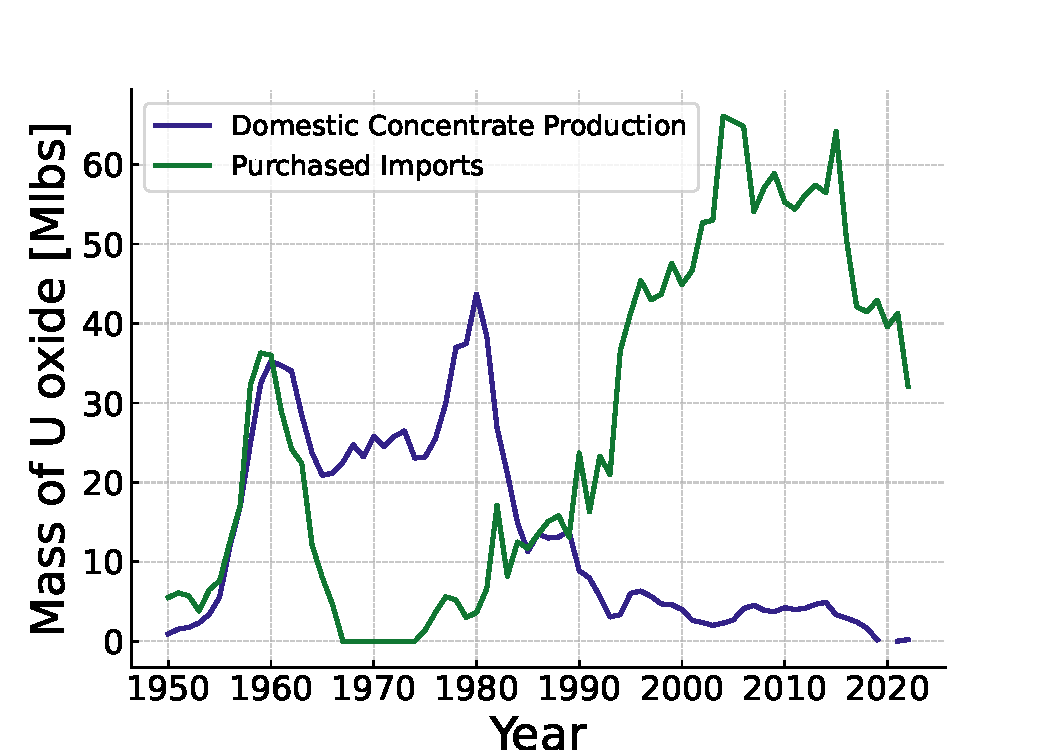
\includegraphics[scale=0.8]{images/intro/uranium_production_imports.pdf}
   \caption{Foregin and domestic uranium purchases over time \cite{eia_monthly_energy_review_2024}.}
   \label{fig:foregin_u3o8}
\end{figure}

% \subsection{Waste}
% How is radioactive waste managed and disposed of?







On a macroscopic level, climate change will drive shorelines to move, permafrost to recede, and congenital ice-sheets to melt. Translating these well-known effects into chemical consequences that dictate the design of a repository will require site-specific adaptations on several fronts. Special attention must be given to the effects in the first few thousand years, as this period will exhibit the highest activity. In the case of meltwater exposure, it is possible that water saturated with dissolved $O_2$ could infiltrate some repositories, potentially altering the oxidizing conditions \cite{gurban_hydrochemical_2001}. Consequently, regulators considering the 100,000-year perspective of a potential repository must account for proximity to such meltwater sources to meet the demands imposed by a changing climate.

It is entirely possible that sites currently experiencing reducing conditions will continue to do so. However, another consideration is how the salinity of groundwater will be influenced by the changing climate. Changes in salinity affect density, which could either exacerbate or mitigate the spread of contaminants in the event of exposure outside the repository \cite{gurban_hydrochemical_2001}. This change in salinity also has the potential to interact differently with canisters, necessitating that proactive regulators ensure containment is designed to withstand a changing environment over the repository's lifetime.

An additional layer of consideration for both of these regulatory concerns is the imminent deployment of new nuclear fuels with different compositions and forms. Some fuels are designed with pyrolytic carbon matrices that can immobilize decay products for much longer than current fuel forms. As new fuel technologies are deployed, it follows that \gls{nfc} facilities will adapt accordingly. These changes, although seemingly slight (the fuel will likely still be uranium-based), can have significant consequences over the course of 100,000 years \cite{hyland_post_closure_2013}.


% How do international treaties and agreements affect nuclear fuel cycle activities?
In the emerging stage of the \gls{nfc}


% What are the prospects for new reactor designs and fuel types?



% What are the main challenges facing the nuclear fuel cycle today?



% What opportunities exist for innovation and improvement in the nuclear fuel cycle?

